\documentclass[11pt]{article}

\usepackage[a4paper,margin=2.5cm]{geometry}
\usepackage{amsmath}
\usepackage{graphicx}
\usepackage{booktabs}
\usepackage{enumitem}
\usepackage[numbers,sort&compress]{natbib}
\usepackage{xcolor}
\usepackage{tikz}
\usetikzlibrary{arrows.meta,calc,fit,positioning,shapes.geometric}
\usepackage[colorlinks=true,linkcolor=blue!55!black,citecolor=blue!55!black,urlcolor=blue!55!black]{hyperref}
\hypersetup{colorlinks=true,linkcolor=blue!55!black,citecolor=blue!55!black,urlcolor=blue!55!black}

\newcommand{\FORGE}{\textsc{Forge-Bench}}
\newcommand{\axis}[1]{\texttt{#1}}
\newcommand{\best}{\textbf}
\newcommand{\second}{\underline}
\newcommand{\tablestyle}[2]{\setlength{\tabcolsep}{#1}\renewcommand{\arraystretch}{#2}\centering\footnotesize}

\title{FORGE-Bench: Factory-Oriented Reasoning and Generation Evaluation for Industrial Video Generation}
\author{Anonymous Authors\\Anonymous Institution}
\date{}

\begin{document}
\maketitle

\begin{abstract}
Recent image-to-video models can synthesize visually compelling clips, yet visual appeal alone is an unreliable indicator of whether an industrial video is physically credible, structurally stable, causally correct, or useful in practice. We introduce \FORGE, a benchmark for evaluating industrial video generation under explicit geometric, physical, temporal, semantic, and application constraints. The benchmark contains 500 image-conditioned tasks spanning 60 scene families in five industrial domains, balanced across domains and stratified into easy, medium, hard, and adversarial tiers. We organize evaluation as an orthogonal domain--task matrix and score five technical axes---industrial logic and fact alignment, geometric integrity, physical plausibility, temporal consistency, and reference-and-motion fidelity---together with a separate application-usefulness axis. The protocol combines a multimodal model judge with task-aware computer-vision evidence, explicit event-completion checks, deterministic frame sampling, and auditable reliability calibration. We release ten matched model-output collections, each containing all 500 tasks (5,000 videos total). Following a 451-video refresh on September 11, 2026, all affected scores are being recomputed under the frozen protocol; superseded pre-refresh scores are not reported as current results. Code, prompts, annotations, references, generated videos, and evaluation artifacts are released to support reproducible research on dependable industrial video generation.
\end{abstract}

\noindent\textbf{Code:} \url{https://github.com/am-ns/FORGE-Bench}\\
\textbf{Dataset:} \url{https://huggingface.co/datasets/aaaabcd/FORGE-Bench}

\begin{figure*}[t]
\centering
\resizebox{\textwidth}{!}{%
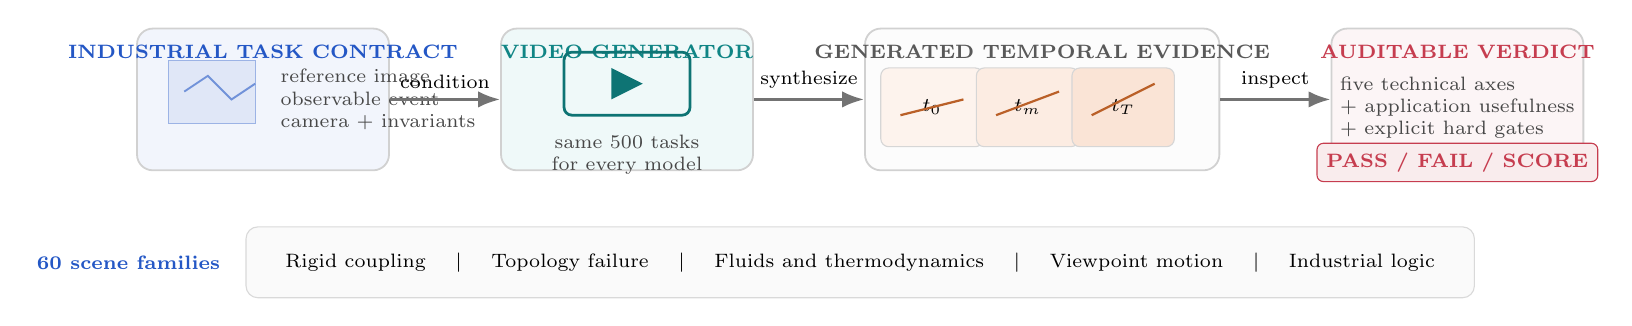
\begin{tikzpicture}[
  font=\sffamily,
  >=Latex,
  card/.style={draw=black!18, rounded corners=2mm, line width=.65pt,
    minimum height=18mm, inner sep=3mm, fill=white},
  stage/.style={card, minimum width=32mm},
  clip/.style={draw=black!16, rounded corners=1mm, minimum width=13mm,
    minimum height=10mm, inner sep=1mm},
  flow/.style={->, line width=1.1pt, draw=black!55},
  label/.style={font=\scriptsize\bfseries, text=black!65},
  note/.style={font=\scriptsize, align=center, text=black!72}
]
\definecolor{forgeblue}{HTML}{2457C5}
\definecolor{forgecyan}{HTML}{14A6A6}
\definecolor{forgeorange}{HTML}{E87832}
\definecolor{forgered}{HTML}{C63D4F}

% Input contract
\node[stage, fill=forgeblue!6] (input) at (0,0) {};
\node[label, text=forgeblue] at ([yshift=6mm]input.center) {INDUSTRIAL TASK CONTRACT};
\draw[fill=forgeblue!14, draw=forgeblue!45] ([xshift=-12mm,yshift=-3mm]input.center)
  rectangle ++(11mm,8mm);
\draw[forgeblue!65, line width=.7pt] ([xshift=-10mm,yshift=1mm]input.center)
  -- ++(3mm,2mm) -- ++(3mm,-3mm) -- ++(3mm,2mm);
\node[note, anchor=west, align=left] at ([xshift=1mm,yshift=0mm]input.center)
  {reference image\\observable event\\camera + invariants};

% Generator
\node[stage, right=14mm of input, fill=forgecyan!7] (gen) {};
\node[label, text=forgecyan!80!black] at ([yshift=6mm]gen.center) {VIDEO GENERATOR};
\draw[draw=forgecyan!70!black, line width=1pt, rounded corners=1mm]
  ([xshift=-8mm,yshift=-2mm]gen.center) rectangle ++(16mm,8mm);
\draw[fill=forgecyan!70!black, draw=none]
  ([xshift=-2mm,yshift=0mm]gen.center) -- ++(0,4mm) -- ++(4mm,-2mm) -- cycle;
\node[note] at ([yshift=-7mm]gen.center) {same 500 tasks\\for every model};

% Generated temporal evidence
\node[card, minimum width=45mm, right=14mm of gen, fill=black!1] (video) {};
\node[label] at ([yshift=6mm]video.center) {GENERATED TEMPORAL EVIDENCE};
\node[clip, fill=forgeorange!9] (f1) at ([xshift=-14mm,yshift=-1mm]video.center) {\scriptsize $t_0$};
\node[clip, fill=forgeorange!14, right=-1mm of f1] (f2) {\scriptsize $t_m$};
\node[clip, fill=forgeorange!20, right=-1mm of f2] (f3) {\scriptsize $t_T$};
\draw[forgeorange!80!black, line width=.8pt] ([xshift=-4mm,yshift=-1mm]f1.center)
  -- ([xshift=4mm,yshift=1mm]f1.center);
\draw[forgeorange!80!black, line width=.8pt] ([xshift=-4mm,yshift=-1mm]f2.center)
  -- ([xshift=4mm,yshift=2mm]f2.center);
\draw[forgeorange!80!black, line width=.8pt] ([xshift=-4mm,yshift=-1mm]f3.center)
  -- ([xshift=4mm,yshift=3mm]f3.center);

% Verdict
\node[stage, right=14mm of video, fill=forgered!5] (score) {};
\node[label, text=forgered] at ([yshift=6mm]score.center) {AUDITABLE VERDICT};
\node[note, align=left] at ([yshift=-1mm]score.center)
  {five technical axes\\+ application usefulness\\+ explicit hard gates};
\node[draw=forgered, rounded corners=.8mm, fill=forgered!10,
  font=\scriptsize\bfseries, text=forgered, inner sep=1.2mm]
  at ([yshift=-8mm]score.center) {PASS / FAIL / SCORE};

\draw[flow] (input) -- node[above, font=\scriptsize] {condition} (gen);
\draw[flow] (gen) -- node[above, font=\scriptsize] {synthesize} (video);
\draw[flow] (video) -- node[above, font=\scriptsize] {inspect} (score);

% Bottom capability strip
\node[draw=black!15, rounded corners=1.5mm, fill=black!2,
  minimum width=156mm, minimum height=9mm, below=7mm of $(input.south)!0.5!(score.south)$,
  font=\scriptsize, align=center] (strip)
  {Rigid coupling \quad $\vert$ \quad Topology failure \quad $\vert$ \quad
   Fluids and thermodynamics \quad $\vert$ \quad Viewpoint motion \quad $\vert$ \quad
   Industrial logic};
\node[anchor=east, font=\scriptsize\bfseries, text=forgeblue] at
  ([xshift=-2mm]strip.west) {60 scene families};
\end{tikzpicture}
}
\caption{\FORGE{} evaluates whether an image-conditioned industrial video executes the requested event while preserving structural, physical, temporal, and application-critical constraints. Unlike perceptual-quality-only evaluation, the benchmark exposes failures through task-specific evidence and auditable gates.}
\label{fig:teaser}
\end{figure*}


\section{Introduction}
\label{sec:intro}

Video generation has progressed from short, weakly controlled clips to systems capable of maintaining recognizable subjects, following camera instructions, and rendering complex motion. Existing benchmarks have played a central role in this progress by decomposing visual quality into interpretable dimensions~\cite{huang2024vbench,huang2025vbenchpp}, measuring broad user-facing quality~\cite{liu2023evalcrafter}, and testing compositional prompt following~\cite{sun2024t2vcompbench}. These evaluations are necessary, but they do not fully characterize the requirements of industrial video.

In an industrial scene, a clip may be sharp and temporally smooth while being functionally wrong. A crane cable can merge into its load; an excavator linkage can change topology; a robot can penetrate a workpiece; smoke may spread against the expected pressure or airflow; or a safety alarm may appear without the triggering event. Such errors are not merely aesthetic. They can invalidate synthetic data, produce misleading training material, or conceal hazards in inspection and operational planning. Consequently, evaluating industrial video requires reasoning about \emph{what changed}, \emph{what remained invariant}, \emph{why the event occurred}, and \emph{whether the resulting clip supports a concrete application decision}.

We introduce \FORGE---\textbf{F}actory-\textbf{O}riented \textbf{R}easoning and \textbf{G}eneration \textbf{E}valuation---to address this gap. The benchmark is designed around two orthogonal views. The first is the scenario domain: visual security, embodied robotics, heavy-load construction, precision-defect generation, and extreme emergency. The second is the abstract capability under test: rigid-body kinematics and coupling, topology mutation and failure, fluid dynamics and thermodynamics, spatial exploration and viewpoint, and industrial logic and compliance. This domain--task matrix separates failures caused by visual context from failures caused by the underlying generative capability.

Each task begins with a reference image and an executable image-to-video prompt. Annotations specify the requested event, camera behavior, terminal state, preserved regions, hard constraints, application objective, and known misleading failure modes. Evaluation uses a five-plus-one structure: five technical axes are aggregated into a task-conditioned technical score, while application usefulness is reported and incorporated as a distinct layer. Task-aware visual operators provide evidence to a multimodal judge rather than silently replacing it, and all hard adjustments are exposed in the output.

The contributions of this work are fourfold:
\begin{itemize}[leftmargin=*]
    \item We formulate industrial video evaluation as an orthogonal matrix of five scenario domains and five abstract task categories, covering 500 annotated tasks across 60 scene families.
    \item We release a balanced 500-task benchmark with one reference image per task, a frozen prompt contract, four difficulty tiers, and explicit application objectives.
    \item We propose an auditable five-plus-one protocol that combines structured multimodal judging, deterministic temporal evidence, task-aware computer-vision operators, observable-event checks, and non-duplicative hard gates.
    \item We benchmark ten representative generators and report rankings, confidence intervals, domain--task breakdowns, difficulty trends, and failure analyses.
\end{itemize}

\section{Related Work}
\label{sec:related}

\paragraph{Video-generation evaluation.}
Early distributional measures such as Fr\'echet Video Distance compare generated and real feature distributions~\cite{unterthiner2018fvd}, but a single corpus-level statistic offers limited diagnostic value for prompt-conditioned generation. VBench decomposes generation quality into multiple perceptual and semantic dimensions and validates them against human preference~\cite{huang2024vbench}; VBench++ extends this framework to image-to-video settings and trustworthiness~\cite{huang2025vbenchpp}. EvalCrafter combines a broad prompt set with objective metrics calibrated to human opinion~\cite{liu2023evalcrafter}. In contrast, \FORGE focuses on industrial correctness: structural invariants, event causality, physical evolution, camera execution, and downstream decision value.

\paragraph{Compositional and reasoning-oriented evaluation.}
T2V-CompBench tests attribute, action, interaction, spatial, and numerical composition using learned and programmatic metrics~\cite{sun2024t2vcompbench}. This direction motivates evaluating more than generic text--video similarity. Industrial prompts, however, contain constraints that are often conditional: a machine should stop \emph{after} a boundary is crossed, a fracture should remain localized, or a load should move while its rigging stays coupled. \FORGE therefore associates each task with observable events, implicit-rule questions, failure modes, and task-specific evidence.

\paragraph{Multimodal judges and hybrid metrics.}
Large multimodal models can describe temporal evidence and apply natural-language rubrics, but their outputs may be sensitive to prompt wording, incomplete visual sampling, and score anchoring. Purely programmatic metrics have the opposite limitation: they are reproducible but capture only a narrow proxy. Our protocol combines the two. A model judge assigns the semantic axis scores, while classical operators expose measurements such as joint drift, regional change, plume continuity, and camera motion. Operator evidence is validity- and confidence-gated and is never counted as an additional independent axis.

\paragraph{Industrial visual understanding.}
Industrial perception research commonly targets a single downstream problem, such as defect inspection, robot manipulation, safety monitoring, or predictive maintenance. \FORGE instead evaluates a generator's ability to produce videos that could plausibly support these workflows. It does not claim that a generated clip is safe for deployment; rather, it measures whether the visual evidence satisfies a frozen industrial task contract and exposes where that contract fails.

\paragraph{Comparison with physics-oriented benchmarks.}
Table~\ref{tab:benchmark-comparison} compares representative physics-oriented video benchmarks by scenario, data source, physical depth, topology-failure coverage, evaluation pipeline, and scoring mechanism. \FORGE differs in targeting high-risk industrial scenarios, explicitly testing topology failures, and combining objective computer-vision operators with multimodal causal question answering under a strict static gate.

\begin{table*}[t]
\centering
\scriptsize
\setlength{\tabcolsep}{2.4pt}
\renewcommand{\arraystretch}{1.12}
\caption{Comparison of representative physics-oriented video benchmarks. Coverage is described as full, partial, or none without symbol-dependent typography.}
\label{tab:benchmark-comparison}
\resizebox{\textwidth}{!}{%
\begin{tabular}{lllllll}
\toprule
Benchmark & Scenario domain & Data source & Physics depth & Topology failure & Evaluation pipeline & Core metric \\
\midrule
PhyGenBench (2025) & High-school physics / common sense & Web images / synthetic & Partial: basic laws & None & VLM visual QA & Weighted mean \\
RigidBench (2026) & Synthetic rigid-body collisions & Blender 3D rendering & Full: rigid trajectories & None & 3D trajectory error & MAE \\
Physion-Eval (2026) & Daily life / human actions & Real-world short videos & Full: daily physics & None & VLM failure detection & Failure rate / aggregate \\
Physics-IQ (2025) & General video dynamics & Generic video clips & Partial: macro dynamics & None & VLM multiple choice & Accuracy \\
VBench-2.0 (2025) & General generation & Generic generations & Partial: shallow intuition & None & Pretrained VLM judge & Mean across dimensions \\
\textbf{\FORGE{} (ours)} & \textbf{Industrial / security / disaster / manufacturing} & \textbf{Surveillance / satellite / BIM / scientific diagrams} & \textbf{Full: extreme dynamics / fluids} & \textbf{Full: targeted} & \textbf{CV operators + VLM causal QA} & \textbf{Strict usability with static veto} \\
\bottomrule
\end{tabular}%
}
\end{table*}

\section{Benchmark Design}
\label{sec:benchmark}

\subsection{Design objectives}

The benchmark follows four principles. First, every sample must specify an observable event rather than a purely stylistic request. Second, the reference image defines visual identity and regions that should remain stable. Third, task annotations must identify at least one meaningful failure mode. Fourth, evaluation must support both a scalar comparison and an explanation localized to a domain, task family, axis, or event.

\subsection{Dataset composition}

The benchmark contains 500 samples from 60 scene families and 500 unique reference images, with exactly 100 tasks from each domain. Tables~\ref{tab:domain-stats} and~\ref{tab:task-stats} summarize the two orthogonal views separately. The task distribution is intentionally non-uniform because not every capability is equally meaningful in every domain; for example, fluid behavior is common in emergency scenarios but absent from the embodied-robotics subset.

\begin{table}[t]
\tablestyle{5pt}{1.12}
\caption{Scenario-domain composition of the 500-task benchmark.}
\label{tab:domain-stats}
\begin{tabular}{lr}
\toprule
Category & Samples \\
\midrule
Visual security & 100 \\
Embodied robotics & 100 \\
Heavy-load construction & 100 \\
Precision-defect generation & 100 \\
Extreme emergency & 100 \\
\bottomrule
\end{tabular}
\end{table}

\begin{table}[t]
\tablestyle{5pt}{1.12}
\caption{Task-category composition of the 500-task benchmark.}
\label{tab:task-stats}
\begin{tabular}{lr}
\toprule
Category & Samples \\
\midrule
Rigid-body kinematics and coupling & 109 \\
Topology mutation and failure & 114 \\
Fluid dynamics and thermodynamics & 83 \\
Spatial exploration and viewpoint & 79 \\
Industrial logic and compliance & 115 \\
\bottomrule
\end{tabular}
\end{table}

\subsection{Scenario domains}

\textbf{Visual security} covers intrusion, personal protective equipment, vehicle--pedestrian interaction, surveillance viewpoints, and alarm response. \textbf{Embodied robotics} covers manipulation, mobile navigation, contact, handover, interlocks, and emergency stopping. \textbf{Heavy-load construction} stresses rigging, crane and excavator kinematics, ground support, alignment, and load-path failures. \textbf{Precision-defect generation} targets localized PCB, weld, gear, connector, seal, and surface defects, together with endoscopic inspection. \textbf{Extreme emergency} covers pressure release, fire, smoke, thermal runaway, structural collapse, evacuation, and containment breach.

\subsection{Task taxonomy}

The five abstract task categories factor capability from setting. Rigid-body tasks require stable joints, supports, contacts, and coupled motion. Topology-mutation tasks require a specified local change while preserving unaffected structure. Fluid and thermodynamic tasks require plausible direction, continuity, diffusion, and interaction with boundaries. Spatial-viewpoint tasks require an explicit orbit, pan, dolly, inspection trajectory, or static-camera condition. Logic-and-compliance tasks require a complete trigger--response--outcome chain.

This factorization yields an interpretable domain--task matrix. Missing cells are meaningful rather than accidental: they indicate capability--domain combinations for which the current benchmark does not define a defensible task. We report both marginal scores and populated cell scores instead of imputing empty cells.

\subsection{Prompt and annotation contract}

Every operational sample provides a compact \texttt{video\_generation\_prompt} and a richer evaluation prompt. The generation prompt identifies the visible event, camera behavior, terminal state, reference-preservation requirement, and prohibited artifacts. The evaluation record further includes hard constraints, required observable events, decision-relevant elements, success criteria, implicit-rule questions, per-axis rubrics, and anticipated misleading failures. Outputs are named \texttt{\{task\_id\}.mp4}, making the mapping from task to model output deterministic.

\subsection{Difficulty stratification}

Difficulty is assigned before model evaluation. The operational split follows a fixed 20/30/30/20 distribution: 100 easy, 150 medium, 150 hard, and 100 adversarial tasks. Difficulty reflects coupled interactions, geometry, viewpoint range, event count, occlusion, physical constraints, and known model weaknesses. ``Easy'' is relative to this industrial benchmark and still requires identity preservation and event completion.

The split contains 182 static-camera, 119 dolly, 101 pan, and 98 orbit tasks. Application targets include emergency rehearsal (125), heavy-operation risk assessment (100), robotic operation (100), safety training (84), inspection and maintenance (58), and defect generation (33).

\section{Evaluation Protocol}
\label{sec:evaluation}

\begin{figure*}[t]
\centering
\resizebox{\textwidth}{!}{%
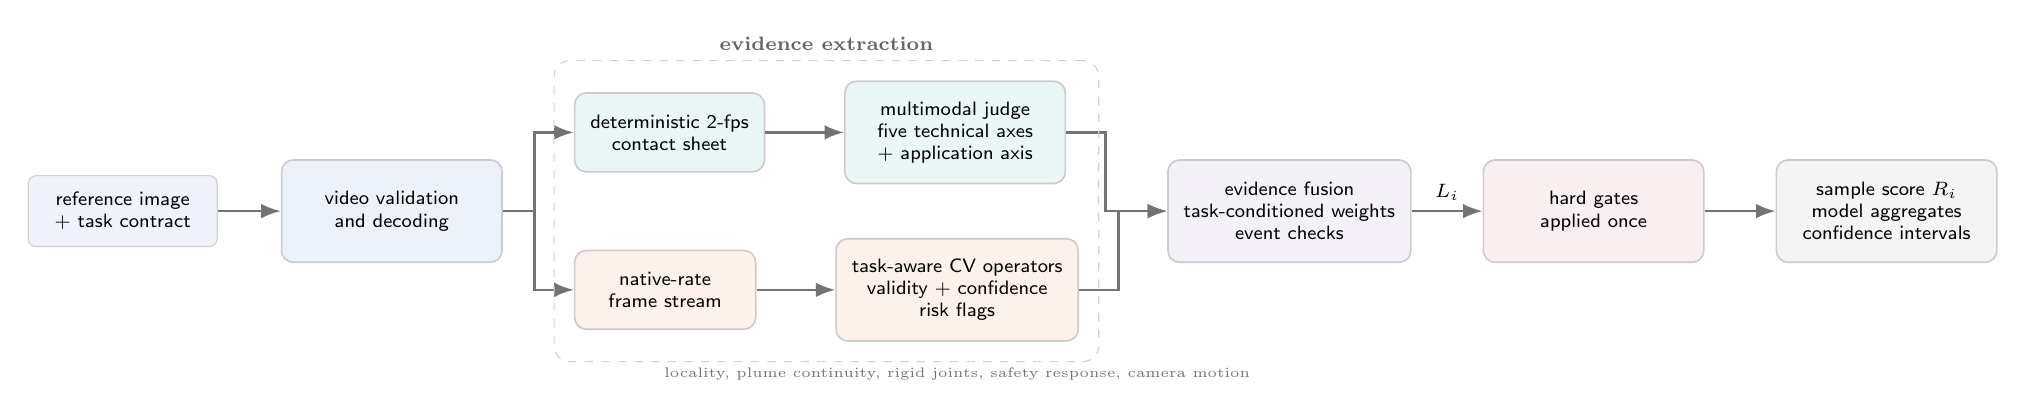
\begin{tikzpicture}[
  font=\sffamily\scriptsize,
  >=Latex,
  block/.style={draw=black!20, rounded corners=1.5mm, line width=.6pt,
    minimum width=28mm, minimum height=13mm, align=center, inner sep=2mm},
  small/.style={block, minimum width=23mm, minimum height=10mm},
  arrow/.style={->, draw=black!55, line width=.9pt},
  data/.style={draw=black!18, rounded corners=1mm, fill=black!2,
    minimum width=24mm, minimum height=9mm, align=center},
  group/.style={draw=black!18, dashed, rounded corners=2mm, inner sep=2.5mm}
]
\definecolor{pblue}{HTML}{2457C5}
\definecolor{pteal}{HTML}{078C8C}
\definecolor{porange}{HTML}{D96A24}
\definecolor{pred}{HTML}{BE3A4A}
\definecolor{ppurple}{HTML}{7354B5}

\node[data, fill=pblue!7] (task) {reference image\\+ task contract};
\node[block, right=8mm of task, fill=pblue!8] (decode) {video validation\\and decoding};

\node[small, right=9mm of decode, yshift=10mm, fill=pteal!8] (sample)
  {deterministic 2-fps\\contact sheet};
\node[small, right=9mm of decode, yshift=-10mm, fill=porange!9] (native)
  {native-rate\\frame stream};

\node[block, right=10mm of sample, fill=pteal!8] (vlm)
  {multimodal judge\\five technical axes\\+ application axis};
\node[block, right=10mm of native, fill=porange!9] (cv)
  {task-aware CV operators\\validity + confidence\\risk flags};

\node[block, right=12mm of $(vlm.east)!0.5!(cv.east)$, fill=ppurple!8] (fusion)
  {evidence fusion\\task-conditioned weights\\event checks};
\node[block, right=9mm of fusion, fill=pred!8] (gate)
  {hard gates\\applied once};
\node[block, right=9mm of gate, fill=black!4] (report)
  {sample score $R_i$\\model aggregates\\confidence intervals};

\draw[arrow] (task) -- (decode);
\draw[arrow] (decode.east) -- ++(4mm,0) |- (sample.west);
\draw[arrow] (decode.east) -- ++(4mm,0) |- (native.west);
\draw[arrow] (sample) -- (vlm);
\draw[arrow] (native) -- (cv);
\draw[arrow] (vlm.east) -- ++(5mm,0) |- (fusion.west);
\draw[arrow] (cv.east) -- ++(5mm,0) |- (fusion.west);
\draw[arrow] (fusion) -- node[above] {$L_i$} (gate);
\draw[arrow] (gate) -- (report);

\node[group, fit=(sample)(native)(vlm)(cv), label={[font=\scriptsize\bfseries,
  text=black!60]above:evidence extraction}] {};
\node[font=\tiny, text=black!55, below=2mm of cv]
  {locality, plume continuity, rigid joints, safety response, camera motion};
\end{tikzpicture}
}
\caption{The \FORGE{} evaluation pipeline. Deterministically sampled evidence supports semantic judging, while native-rate frames support task-aware computer-vision operators. Validated evidence is fused without double counting; explicit gates produce an auditable ranking score and diagnostics.}
\label{fig:evaluation-pipeline}
\end{figure*}


\subsection{Five technical axes plus application usefulness}

For sample $i$, the judge produces five technical scores $s_{i,a}\in[0,100]$: industrial logic and fact alignment, geometric integrity, physical plausibility, temporal consistency, and reference-and-motion fidelity. Application usefulness $u_i\in[0,100]$ is evaluated separately because a technically plausible clip can still fail its intended workflow.

Let $w_{i,a}$ denote the normalized axis weight determined by the task category. The technical score is
\begin{equation}
T_i = \sum_{a=1}^{5} w_{i,a}s_{i,a}, \qquad \sum_{a=1}^{5}w_{i,a}=1.
\end{equation}
Let $c_i\in[0,1]$ be required-event coverage and $m_i\in[0,1]$ the validated required-motion score when applicable. We use continuous reliability functions
\begin{equation}
g_e(c_i)=0.05+0.95c_i^{1.7},\qquad g_m(m_i)=0.25+0.75m_i^{1.2}.
\end{equation}
Event reliability calibrates only industrial logic/fact alignment, reference-and-motion fidelity, and application usefulness; motion reliability calibrates only reference-and-motion fidelity. A verified severe safety failure applies a reliability of 0.5 to industrial logic/fact alignment and application usefulness. After recomputing the weighted technical score $\widetilde T_i$ and calibrated application score $\widetilde u_i$, the single linear five-plus-one score is
\begin{equation}
P_i=0.8\widetilde T_i+0.2\widetilde u_i,\qquad
R_i=\mathrm{clip}_{[0,100]}\!\left(100\frac{P_i-b}{100-b}\right),\quad b=15.
\end{equation}
The fixed $b=15$ represents a preregistered degenerate-generation baseline; the affine transform preserves ordering above the floor and maps a perfect score to 100. There are no post-total 0/30/40 caps. Each semantic multiplier is applied once and recorded in a per-sample ledger. Aggregate ranking is the mean over samples with all required axes, with cluster-bootstrap confidence intervals. No alternative total is used for leaderboard ranking.

\subsection{Temporal evidence and multimodal judging}

The protocol decodes every valid video and retains native-rate frames for continuous computer-vision checks. The multimodal judge receives a deterministic 2-fps view with first/last-frame coverage and audited source indices. In the current Qwen3-VL-235B deployment, chronological frames are assembled into a numbered contact sheet to satisfy the server's one-image-per-request limit without dropping the sampled evidence. Temperature is fixed to zero, the model identifier is frozen, and each axis requires structured JSON containing a score, reasoning, failure modes, confidence, and evidence-frame indices.

\subsection{Operator evidence}

Five operator families complement the judge:
\begin{itemize}[leftmargin=*]
    \item \textbf{Local-region locking} tests whether a requested local defect remains localized instead of regenerating the full scene.
    \item \textbf{Fluid/plume continuity} measures area evolution and centroid continuity for leaks, smoke, fire, spray, and pressure release.
    \item \textbf{Rigid-joint tracking} estimates camera-compensated pairwise drift and spatial track coverage.
    \item \textbf{Safety-response motion} provides weak evidence for stopping or slowing in compliance tasks.
    \item \textbf{Viewpoint motion fidelity} measures orbit, pan, dolly, and static-camera execution.
\end{itemize}
Operators produce evidence and risk flags. A measurement can calibrate its corresponding axis only when its applicability, validity, and confidence conditions are met. This avoids both double-counting and using a fragile proxy as an unconditional score.

\subsection{Application and reasoning checks}

Application usefulness requires visible completion of decision-critical events. For example, an emergency clip must show the relevant trigger and response rather than merely an alarming appearance. Each sample can also provide binary implicit-rule questions. Their accuracy forms a reasoning-alignment diagnostic but does not replace the five-plus-one score.

\subsection{Validity and reproducibility}

Missing videos, undecodable videos, malformed judge responses, missing required axes, and score-floor usage are surfaced explicitly. They are never silently imputed. A model output rejected before evaluation is recorded as such and retained in the 500-task denominator. Reports store hashes of the sample manifest, scoring configuration, evaluation code, and judge configuration, as well as library versions and sampling metadata.

\section{Experiments}
\label{sec:experiments}

\subsection{Experimental setup}

We assemble ten image-to-video systems: HunyuanVideo 1.5, HunyuanVideo 1.5 Distill, MiniMax H3, Kling 3.0 Standard, Seedance 2.5, Veo 3.1 Fast, CogVideoX 1.5, Wan 2.1, Wan 2.2, and Wan 3.0. Each system has the same 500 reference-image/task pairs and frozen generation-facing prompts, yielding 5,000 published videos. Videos are mapped by task identifier and decoded under a common evaluation pipeline. A previously evaluated candidate set is excluded from publication because its generation provenance cannot be verified independently; none of its videos or scores contribute to the results below.

The formal judge is Qwen3-VL-235B-A22B-Instruct-FP8, served with four-GPU tensor parallelism. Four deterministic data shards are evaluated concurrently. Every released model collection contains exactly 500 videos; Seedance task \texttt{erob\_190} is now present. On September 11, 2026, 451 videos across nine collections were refreshed (50 per collection and 51 for Seedance). Under the frozen-cache policy, this invalidates pre-refresh scores for the affected collections and requires complete re-evaluation before publication.

\subsection{Main results}

Table~\ref{tab:main-results} reports results confirmed by canonical aggregate JSON files. A dash denotes a system without a complete aggregate; partial-sample scores are not substituted for complete results.

\begin{table*}[t]
\tablestyle{4pt}{1.1}
\caption{Current evaluation status on the refreshed 500-task operational split. Dashes indicate that post-refresh complete aggregates are pending; superseded pre-refresh values are intentionally omitted.}
\label{tab:main-results}
\resizebox{\textwidth}{!}{%
\begin{tabular}{lrrrrrrr}
\toprule
Model & \shortstack{Industrial logic and\\fact alignment} & \shortstack{Geometric\\integrity} & \shortstack{Physical\\plausibility} & \shortstack{Temporal\\consistency} & \shortstack{Reference and\\motion fidelity} & \shortstack{Application\\usefulness} & \shortstack{Ranking\\score} \\
\midrule
HunyuanVideo 1.5 & -- & -- & -- & -- & -- & -- & -- \\
HunyuanVideo 1.5 Distill & -- & -- & -- & -- & -- & -- & -- \\
MiniMax H3 & -- & -- & -- & -- & -- & -- & -- \\
Kling 3.0 Standard & -- & -- & -- & -- & -- & -- & -- \\
Seedance 2.5 & -- & -- & -- & -- & -- & -- & -- \\
Veo 3.1 Fast & -- & -- & -- & -- & -- & -- & -- \\
CogVideoX 1.5 & -- & -- & -- & -- & -- & -- & -- \\
Wan 2.1 & -- & -- & -- & -- & -- & -- & -- \\
Wan 2.2 & -- & -- & -- & -- & -- & -- & -- \\
Wan 3.0 & -- & -- & -- & -- & -- & -- & -- \\
\bottomrule
\end{tabular}
}
\end{table*}

No post-refresh model currently has a complete aggregate that is valid for publication. The table therefore reports no point estimates or confidence intervals. Historical aggregates produced before the video refresh remain useful only as pipeline diagnostics and are not comparable to the current Hugging Face release. Rankings, cluster-bootstrap confidence intervals, and axis-level comparisons will be restored only after every model has been evaluated against the current 500-file inventory and passes \texttt{ranking\_publishable=true}.

\paragraph{Analysis framework.}
The analysis asks whether generic visual coherence guarantees industrial performance, how scores change with difficulty, and which capability-specific trade-offs are hidden by a single mean.

\subsection{Domain and task breakdown}

Domain--task analysis uses a $5\times5$ matrix and macro averages over populated cells. It distinguishes general geometry weaknesses from failures concentrated in periodic precision structures and separates fluid-evolution errors from causal incompleteness in emergency scenes.

\subsection{Difficulty and application breakdown}

Results are stratified by the four preassigned difficulty tiers and six application types. The analysis considers not only score decline but also which axis first becomes limiting as task complexity rises. Application reporting separately measures required-event coverage and strict application pass rate.

\subsection{Qualitative failure analysis}

Qualitative analysis focuses on cases where conventional visual quality and \FORGE{} disagree: (i) smooth but static clips that omit required camera motion; (ii) visually dramatic failures with impossible topology; (iii) plausible single frames with broken temporal identity; (iv) localized defect prompts that trigger global regeneration; and (v) safety scenarios missing a trigger, response, or terminal state. Reference images, chronological evidence frames, per-axis scores, gate reasons, and judge evidence jointly localize these industrial failures.

\subsection{Limitations}

The benchmark is finite and does not cover every industrial sector, geographic standard, or equipment type. Some physical properties cannot be inferred reliably from pixels alone. Multimodal judges can be biased or inconsistent even under deterministic decoding, and contact-sheet evidence compresses temporal information. The operational split is balanced by domain rather than by real deployment frequency. Finally, benchmark scores indicate conformance to annotated visual contracts, not certification of safety, engineering correctness, or legal compliance.

\section{Conclusion}
\label{sec:conclusion}

We presented \FORGE, a benchmark for industrial image-to-video generation that places structural, physical, causal, temporal, and application correctness alongside conventional visual quality. Its domain--task matrix, 500-task operational split, five-plus-one score, task-aware evidence operators, and explicit validity reporting are intended to make model comparisons both reproducible and actionable. The benchmark asks a stricter question than whether a clip looks realistic: does it preserve the right structure, execute the requested event and camera behavior, obey visible physical constraints, and support the intended industrial decision?

The final version will report ten-model results from the frozen Qwen3-VL-235B protocol, calibrated confidence intervals, and qualitative failure cases. We hope \FORGE{} supports development of video generators whose outputs are not only compelling, but also dependable enough to study in high-consequence industrial workflows.


\bibliographystyle{plainnat}
\bibliography{references}

\clearpage
\appendix
\section{Additional Benchmark Details}

\subsection{Operational split counts}

The 500-task split contains 109 rigid-body kinematics and coupling tasks, 114 topology mutation and failure tasks, 83 fluid dynamics and thermodynamics tasks, 79 spatial exploration and viewpoint tasks, and 115 industrial logic and compliance tasks. Difficulty tiers contain 100 easy, 150 medium, 150 hard, and 100 adversarial samples.

\subsection{Result-completion checklist}

Before submission, the following red placeholders must be replaced from machine-readable artifacts:
\begin{itemize}[leftmargin=*]
    \item main ranking scores and 95\% bootstrap confidence intervals;
    \item per-axis, per-domain, per-task, and domain--task cell means;
    \item strict pass, all-critical-pass, and application-event coverage rates;
    \item rejected, missing-axis, malformed-response, and hard-cap counts;
    \item qualitative figure references and final author metadata.
\end{itemize}

\subsection{Reproducibility record}

The final artifact should record the exact Git commit, sample-manifest SHA-256, scoring-configuration SHA-256, judge model identifier, serving configuration, frame-sampling protocol, dependency versions, and per-model video inventory. The formal protocol uses Qwen3-VL-235B-A22B-Instruct-FP8 with deterministic decoding and four concurrent shards.

\end{document}
